% IUC LaTeX Thesis Template Manual
% Companion to the IUC Thesis & Dissertation Style Manual, Edition 3.0.
% Design follows the Style Manual: cover, serif body, running header,
% annotated 50% page samples, checklist form, back cover.
%
% Build:  cd docs/manual && latexmk -xelatex iuc-template-manual.tex
\documentclass[11pt,a4paper]{article}

% ---------------------------------------------------------------------------
% Page, fonts, colours
% ---------------------------------------------------------------------------
\usepackage[a4paper,top=28mm,bottom=27mm,left=30mm,right=25mm,
  headheight=14pt,headsep=8mm,footskip=14mm]{geometry}
\usepackage{fontspec}
\setmainfont{Latin Modern Roman}
\setsansfont{Latin Modern Sans}
\setmonofont{Latin Modern Mono}
\usepackage[british]{babel}
\usepackage{xcolor}
\definecolor{iucpurple}{HTML}{5A2D82}
\definecolor{iucdeep}{HTML}{4D2470}
\definecolor{iucteal}{HTML}{2D6268}
\definecolor{iucgold}{HTML}{D9B96E}
\definecolor{iucrose}{HTML}{C58A73}
\definecolor{iuccream}{HTML}{F7F0E3}
\definecolor{iuclav}{HTML}{F2F0F5}
\definecolor{iuctealbg}{HTML}{E9EFEF}
\definecolor{iucgrey}{HTML}{5F5A66}
\definecolor{codebg}{HTML}{F7F5FA}

\usepackage{graphicx}
\graphicspath{{img/}}
\usepackage{tikz}
\usetikzlibrary{positioning,arrows.meta,calc,shadows,decorations.pathreplacing}
\usepackage[most]{tcolorbox}
\usepackage{listings}
\usepackage{enumitem}
\usepackage{array,tabularx,booktabs,colortbl,longtable}
\usepackage{titlesec}
\usepackage{fancyhdr}
\usepackage{eso-pic}
\usepackage{amssymb}
\usepackage{caption}
\usepackage{microtype}
\usepackage[hidelinks]{hyperref}
\hypersetup{pdftitle={IUC LaTeX Thesis Template Manual},
  pdfsubject={Companion to the IUC Thesis and Dissertation Style Manual}}

\setlength\parindent{0pt}
\setlength\parskip{6pt}
\setlength\emergencystretch{3em}
\renewcommand\arraystretch{1.2}
\setlist{itemsep=4pt,topsep=4pt}
\setlist[itemize]{label=\textbullet,leftmargin=2.2em}
\setlist[enumerate]{leftmargin=2.2em}

\newcommand\repourl{https://github.com/fahimroslan/iucstyle_latex}
\newcommand\repo{\href{\repourl}{\texttt{github.com/fahimroslan/iucstyle\_latex}}}

% ---------------------------------------------------------------------------
% Headings, captions, lists (as in the Style Manual)
% ---------------------------------------------------------------------------
\titleformat{\section}{\normalfont\Large\bfseries}{\thesection}{0.8em}{}
\titlespacing*{\section}{0pt}{18pt}{10pt}
\titleformat{\subsection}{\normalfont\large\bfseries}{\thesubsection}{0.8em}{}
\titlespacing*{\subsection}{0pt}{14pt}{6pt}
\titleformat{\subsubsection}{\normalfont\normalsize\bfseries}{}{0pt}{}
\titlespacing*{\subsubsection}{0pt}{10pt}{3pt}
\setcounter{secnumdepth}{2}
\setcounter{tocdepth}{2}

\captionsetup{labelfont=bf,labelsep=colon,skip=6pt}
\captionsetup[table]{font=small,position=top}
\renewcommand\listfigurename{List of Figures and Page Samples}

% ---------------------------------------------------------------------------
% Running header and right-edge strip
% ---------------------------------------------------------------------------
\pagestyle{fancy}
\fancyhf{}
\fancyhead[L]{\small IUC LaTeX Thesis Template Manual}
\fancyhead[R]{\small Template Companion Guide}
\fancyfoot[C]{\thepage}
\renewcommand\headrulewidth{0.5pt}
\fancypagestyle{plain}{}

\newif\ifiucstrip \iucstriptrue
\AddToShipoutPictureBG{%
  \ifiucstrip
  \begin{tikzpicture}[remember picture,overlay,x=1mm,y=1mm]
    \shade[left color=white,right color=iucpurple!14]
      ($(current page.south east)+(-12,0)$) rectangle (current page.north east);
    \draw[iucpurple!35,line width=0.5pt]
      ($(current page.south east)+(-7,0)$) -- ($(current page.north east)+(-7,0)$);
    \draw[iucpurple!18,line width=2pt]
      ($(current page.south east)+(-4,0)$) -- ($(current page.north east)+(-4,0)$);
    \draw[iucrose,line width=0.8pt]
      ($(current page.south east)+(-7,24)$) -- ($(current page.south east)+(0,24)$);
  \end{tikzpicture}%
  \fi}

% ---------------------------------------------------------------------------
% Inline helpers
% ---------------------------------------------------------------------------
\newcommand\cmd[1]{\texttt{\textbackslash #1}}
\newcommand\file[1]{\texttt{#1}}
\newtcbox{\ui}{on line,colback=iuclav,colframe=iucpurple!40,boxrule=0.4pt,arc=2pt,
  boxsep=0pt,left=3pt,right=3pt,top=1.5pt,bottom=1pt,
  fontupper=\sffamily\small\bfseries\color{iucdeep}}
\newcommand\then{\,\textrightarrow\,}
\newcommand\cbox{$\square$}

% ---------------------------------------------------------------------------
% Cards, callouts, prompt boxes, code
% ---------------------------------------------------------------------------
\newcommand\cardhead[1]{{\color{iucteal}\rule[-2.5pt]{1.8pt}{12pt}}\hspace{5pt}%
  {\sffamily\bfseries\color{iucpurple}#1}}
\newtcolorbox{card}[1]{enhanced,colback=iuclav,colframe=iucpurple!12,boxrule=0.5pt,
  arc=4pt,left=8pt,right=8pt,top=6pt,bottom=6pt,fontupper=\sffamily\small,
  before upper={\cardhead{#1}\par\smallskip}}

\tcbset{iucnote/.style={enhanced,boxrule=0pt,arc=2pt,left=9pt,right=9pt,top=6pt,
  bottom=6pt,before skip=8pt,after skip=8pt}}
\newtcolorbox{tipbox}[1][Tip]{iucnote,colback=iuctealbg,
  borderline west={3pt}{0pt}{iucteal},
  before upper={\textbf{\sffamily\color{iucteal}#1.}\enspace}}
\newtcolorbox{warnbox}[1][Important]{iucnote,colback=iuccream,
  borderline west={3pt}{0pt}{iucrose},
  before upper={\textbf{\sffamily\color{iucrose!75!black}#1.}\enspace}}
\newtcolorbox{promptbox}[1]{enhanced,colback=iuccream,colframe=iucgold,boxrule=0.6pt,
  arc=3pt,left=9pt,right=9pt,top=5pt,bottom=5pt,before skip=6pt,after skip=6pt,
  title={\sffamily\bfseries\small #1},colbacktitle=iucdeep,coltitle=white,
  toptitle=2pt,bottomtitle=2pt,fontupper=\itshape}

\lstdefinestyle{iuc}{language=[LaTeX]TeX,basicstyle=\ttfamily\small,
  texcsstyle=*\color{iucpurple}\bfseries,commentstyle=\color{iucgrey}\itshape,
  columns=fullflexible,keepspaces=true,showstringspaces=false,breaklines=true,
  upquote=true,
  moretexcs={textcite,parencite,addbibresource,printreferences,tablenote,
    figuresource,eqtitle,makecover,maketitlepage,makedeclaration,keywords,
    matricno,address,degree,degreeabbr,submissiondate,submissionyear,declarationdate,
    institution,toprule,midrule,bottomrule,mainmatter,frontmatter,
    listofequations,listofappendices}}
\lstdefinestyle{plain}{basicstyle=\ttfamily\small,columns=fullflexible,
  keepspaces=true,breaklines=true,upquote=true}
% (no optional argument: a look-ahead for "[" would swallow the first line)
\tcbset{iuccode/.style={enhanced,listing only,colback=codebg,colframe=iucpurple!22,
  boxrule=0.5pt,arc=3pt,left=8pt,right=8pt,top=3pt,bottom=3pt,
  before skip=6pt,after skip=8pt}}
\newtcblisting{code}{iuccode,listing options={style=iuc}}
\newtcblisting{bib}{iuccode,listing options={style=plain}}
\newtcblisting{shell}{iuccode,colback=iucdeep,colframe=iucdeep,
  listing options={style=plain,basicstyle=\ttfamily\small\color{white}}}
\newtcblisting{prompttext}{iuccode,colback=iuccream,colframe=iucgold,
  listing options={style=plain}}

% Panel heading used above page samples and diagrams
\newcommand\panelhead[2]{%
  \noindent{\sffamily\bfseries\color{iucpurple}\MakeUppercase{#1}}\hfill
  {\sffamily\bfseries\footnotesize\color{iucpurple}\MakeUppercase{#2}\hspace*{14mm}}\par
  \vspace{-3pt}{\color{iucgold!80!black}\rule{\linewidth}{0.6pt}}\par\vspace{4pt}}

% ---------------------------------------------------------------------------
% Page samples (50% scale, 105 x 148.5 mm) with numbered source notes
% ---------------------------------------------------------------------------
% \samplepage{page}{text-area: left/top/right/bottom in mm}
\newcommand\samplepage[2]{%
  \node[anchor=north west,inner sep=0pt,draw=black,line width=0.4pt] (pg) at (0,0)
    {
\includegraphics[page=#1,width=105mm]{sample-pages}};
  \def\ta{#2}%
  \foreach \l/\t/\r/\b in \ta {
    \draw[iucpurple!70,dashed,line width=0.4pt] (\l,-\t) rectangle (\r,-\b);}
  \fill[iuclav,rounded corners=3pt] (111,0) rectangle (155,-148.5);}
% \snote{number}{y of note}{title}{text}{target x,y}
\newcommand\snote[5]{%
  \node[circle,fill=iucpurple,text=white,font=\sffamily\bfseries\scriptsize,
    inner sep=0pt,minimum size=4mm] (n#1) at (115,#2) {#1};
  \node[anchor=north west,text width=35mm,align=left,inner sep=0pt,
    font=\sffamily\scriptsize] at (118.5,#2+1.6)
    {\textbf{\color{iucdeep}#3}\\[1pt]#4};
  \draw[iucpurple,line width=0.45pt,-{Stealth[length=1.8mm,width=1.4mm]}]
    (n#1.west) -- (#5);}
\newcommand\samplescale{%
  \node[anchor=north west,font=\sffamily\tiny,text=iucgrey] at (0,-150.5)
    {50\% scale: A4 page = 105 $\times$ 148.5 mm. Dashed lines mark the text area.};}

% Table header cell
\newcommand\thd[1]{\bfseries #1}

\begin{document}

% ===========================================================================
% Cover
% ===========================================================================
\iucstripfalse
\thispagestyle{empty}
\begin{tikzpicture}[remember picture,overlay,x=1mm,y=1mm]
  \coordinate (NW) at (current page.north west);
  \coordinate (SW) at (current page.south west);
  \coordinate (SE) at (current page.south east);
  \fill[iucdeep] (SW) rectangle (current page.north east);
  \fill[iucpurple] (NW) rectangle ($(current page.north east)+(0,-70)$);
  % teal diagonal
  \fill[iucteal] ($(SE)+(0,210)$) -- (SE) -- ($(SW)+(90,0)$) -- cycle;
  \draw[white!70!iucteal,line width=0.3pt] ($(SE)+(0,210)$) -- ($(SW)+(90,0)$);
  % stripes
  \fill[iucgold] ($(NW)+(18,-70)$) rectangle ($(NW)+(152,-71.4)$);
  \fill[iucteal!85!white] ($(NW)+(152,-70)$) rectangle ($(NW)+(178,-71.4)$);
  \fill[iucrose] ($(NW)+(178,-70)$) rectangle ($(NW)+(191,-71.4)$);
  % logo
  \node[anchor=north west,inner sep=0pt] at ($(NW)+(18,-18)$)
    {
\includegraphics[width=125mm]{iuc-logo-white}};
  % title block
  \fill[iucgold] ($(NW)+(26,-96)$) rectangle ($(NW)+(27.6,-163)$);
  \node[anchor=north west,text=iucgold,font=\sffamily\bfseries\small]
    at ($(NW)+(34,-95)$) {\addfontfeatures{LetterSpace=4}LATEX TEMPLATE AND WORKFLOWS};
  \node[anchor=north west,align=left,text=white,
    font=\sffamily\bfseries\fontsize{30}{34}\selectfont]
    at ($(NW)+(33,-104)$) {\addfontfeatures{LetterSpace=3}THESIS TEMPLATE\\
      \addfontfeatures{LetterSpace=3}USER MANUAL};
  \node[anchor=north west,text=white,font=\sffamily\large]
    at ($(NW)+(34,-129)$) {Guide for Candidates, Supervisors, and Programme Staff};
  % illustration: laptop with LaTeX source and a typeset page
  \begin{scope}[shift={($(SE)+(-72,98)$)}]
    \fill[black,opacity=0.22] (0,-27) ellipse (52 and 4);
    % laptop base
    \fill[iuccream] (-44,-24) -- (44,-24) -- (38,-19) -- (-38,-19) -- cycle;
    \draw[iucgold,line width=0.8pt] (-44,-24) -- (44,-24) -- (38,-19) -- (-38,-19) -- cycle;
    \fill[iucgold!70!black] (-10,-24) rectangle (10,-23);
    % screen
    \fill[iucgold,rounded corners=2pt] (-37,-19) rectangle (37,30);
    \fill[iucdeep!80!black,rounded corners=1pt] (-34.5,-16.5) rectangle (34.5,27.5);
    \node[anchor=north west,font=\ttfamily\tiny,text=iucgold,align=left,inner sep=0pt]
      at (-31,24.5) {\textbackslash chapter\{Introduction\}};
    \node[anchor=north west,font=\ttfamily\tiny,text=white!80,align=left,inner sep=0pt]
      at (-31,18.5) {\textbackslash section\{Purpose\}};
    \foreach \y/\w in {12/48,8/54,4/40,0/50,-4/30}
      \fill[iucteal!70!white] (-31,\y) rectangle ({-31+\w},{\y+1.4});
    \node[anchor=north west,font=\ttfamily\tiny,text=iucrose!80!white,inner sep=0pt]
      at (-31,-7.5) {\textbackslash parencite\{smith2023\}};
    % typeset page coming out of the screen
    \begin{scope}[shift={(40,6)},rotate=-9]
      \fill[black,opacity=0.25] (-15.5,-25.5) rectangle (17,22);
      \fill[white] (-17,-24) rectangle (15.5,23.5);
      \node[font=\bfseries\tiny,text=iucdeep] at (-0.8,18.5) {CHAPTER 1};
      \node[font=\bfseries\tiny,text=iucdeep] at (-0.8,14.8) {INTRODUCTION};
      \foreach \y in {9,5.5,2,-1.5,-5,-8.5,-12,-15.5}
        \fill[iucpurple!30] (-13,\y) rectangle (11.5,{\y+1.2});
      \node[font=\tiny,text=iucgrey] at (-0.8,-21) {1};
    \end{scope}
    % sparkles
    \foreach \p in {(-48,34),(52,38),(60,-6)}
      \node[text=iucgold,font=\large] at \p {+};
  \end{scope}
  % edition card
  \fill[iuccream,rounded corners=6pt] ($(SW)+(18,28)$) rectangle ($(SW)+(165,67)$);
  \node[anchor=north west,text=iucdeep,font=\sffamily\bfseries\small]
    at ($(SW)+(27,60)$) {EDITION 1.0\qquad\textbar\qquad ISSUED 27 NOVEMBER 2026};
  \node[anchor=north west,text=iucteal,font=\sffamily\small,text width=130mm]
    at ($(SW)+(27,49)$)
    {Companion to the IUC Thesis \& Dissertation Style Manual, Edition 3.0\\[3pt]
     \texttt{github.com/fahimroslan/iucstyle\_latex}};
  \node[anchor=south east,text=white,font=\sffamily\scriptsize]
    at ($(SE)+(-18,14)$) {INNOVATIVE UNIVERSITY COLLEGE};
  \fill[iucrose] (SW) rectangle ($(SE)+(0,3.5)$);
\end{tikzpicture}
\clearpage
\iucstriptrue

% ===========================================================================
% Front matter
% ===========================================================================
\pagenumbering{roman}
\tableofcontents
\clearpage
\listoftables
\clearpage
\listoffigures
\clearpage
\pagenumbering{arabic}

% ===========================================================================
\section{Purpose of this manual}
% ===========================================================================

This manual explains how to produce an IUC thesis, dissertation, or research
project with the \textbf{IUC LaTeX thesis template}. It is a companion to the
\emph{IUC Thesis \& Dissertation Style Manual}, Edition~3.0. The Style Manual
states the formatting rules; this manual shows how the template applies them
and how to work with it, by hand or with AI tools.

The template implements the Style Manual's layout, typography, pagination,
contents and lists, captions, APA~7 references, appendices, cover, title page,
and spine. Candidates supply the content and their registered details.

If this manual and the Style Manual ever differ, the Style Manual is the
authority. Report the difference on the template's GitHub page under
\ui{Issues} so it can be corrected.

\subsubsection*{Reading the illustrations}

Each page sample is a real page produced by the template, reduced uniformly to
50\%. Dashed lines mark the text area. Numbered notes sit beside the page, with
arrows pointing to the matching feature, and name the \emph{source file and
command} that produces it. Code is printed in a monospaced font, for example
\cmd{chapter}\{Introduction\}. Buttons and menus in software are shown like
\ui{this}.

\subsection{Who should use this manual}

\begin{itemize}
  \item \textbf{Candidates} writing a master's or doctoral thesis, dissertation,
        or research project. No previous LaTeX experience is assumed.
  \item \textbf{Supervisors} who want to understand how their candidates'
        manuscripts are built, or to review them on GitHub.
  \item \textbf{Programme and library staff} who support candidates and check
        manuscripts before submission.
\end{itemize}

\subsection{Candidate responsibility}

The template sets the layout. Candidates remain responsible for:

\begin{itemize}
  \item entering personal, programme, degree, and submission details exactly as
        registered;
  \item the academic content, its accuracy, and its integrity, including any
        text, code, or references produced with AI tools;
  \item meeting the compulsory minimum word count for the study mode
        (Style Manual, Section~3); the template does not count words;
  \item checking every reference against its source; and
  \item reviewing every page of the final PDF before submission.
\end{itemize}

% ===========================================================================
\section{The template at a glance}
% ===========================================================================

\begin{figure}[htbp]
\begin{tcbraster}[raster columns=2,raster equal height=rows,raster column skip=9pt,
  raster row skip=9pt]
\begin{card}{What you edit}
  \textbf{Text files only:} your details in \file{metadata.tex}, chapters in
  \file{chapters/}, references in \file{references.bib}.\par
  The formatting file \file{iucthesis.cls} is never edited.
\end{card}
\begin{card}{What it formats}
  \textbf{Layout:} A4, IUC margins, 40~mm chapter openings.\par
  \textbf{Text:} Times New Roman 12~pt, double spacing, IUC headings.
\end{card}
\begin{card}{What it generates}
  Cover, title page, declaration, contents page, and lists of tables, figures,
  equations, and appendices, with Roman and Arabic page numbers.
\end{card}
\begin{card}{References}
  \textbf{APA 7th edition} citations and reference list from a
  \file{.bib} file, sorted and formatted automatically.
\end{card}
\begin{card}{Ways to work}
  \textbf{Online:} Overleaf or GitHub.\par
  \textbf{Offline:} VS Code, TeXstudio, or the command line.\par
  \textbf{Assisted:} Claude and other AI tools.
\end{card}
\begin{card}{Engine and licence}
  \textbf{XeLaTeX} with \textbf{biber}; pdfLaTeX is not supported.\par
  Free and open: LaTeX Project Public License 1.3c.
\end{card}
\end{tcbraster}
\caption{The template at a glance.}
\label{fig:glance}
\end{figure}

\textbf{What the template does not do.} It does not count words, judge academic
quality, or check that references exist. The binder applies the cover colour
(purple for master's awards, black for doctoral awards) and the gold lettering;
the template's cover page in the PDF is white.

% ===========================================================================
\section{Choosing a workflow}
% ===========================================================================

All workflows use the same files and produce the same PDF. Choose the one that
suits your equipment and confidence; you can change later.

\begin{table}[htbp]
\caption{The four workflows compared.}
\label{tab:paths}
\small
\begin{tabularx}{\textwidth}{@{}p{28mm}XXp{15mm}p{13mm}@{}}
\toprule
\thd{Workflow} & \thd{How it works} & \thd{Best for} & \thd{Install} & \thd{Effort} \\
\midrule
A.\ Overleaf        & Edit and build in a web browser             & First-time LaTeX users             & Nothing & Low \\
B.\ Own computer    & Free LaTeX system and an editor             & Long-term or offline work          & 4 GB    & Medium \\
C.\ GitHub online   & Edit on github.com; PDF built automatically & Backups and version history        & Nothing & Medium \\
D.\ AI assistant    & Describe changes; AI writes the LaTeX       & Anyone; combines with A, B, or C   & Nothing & Low \\
\bottomrule
\end{tabularx}
\end{table}

\begin{figure}[htbp]
\centering
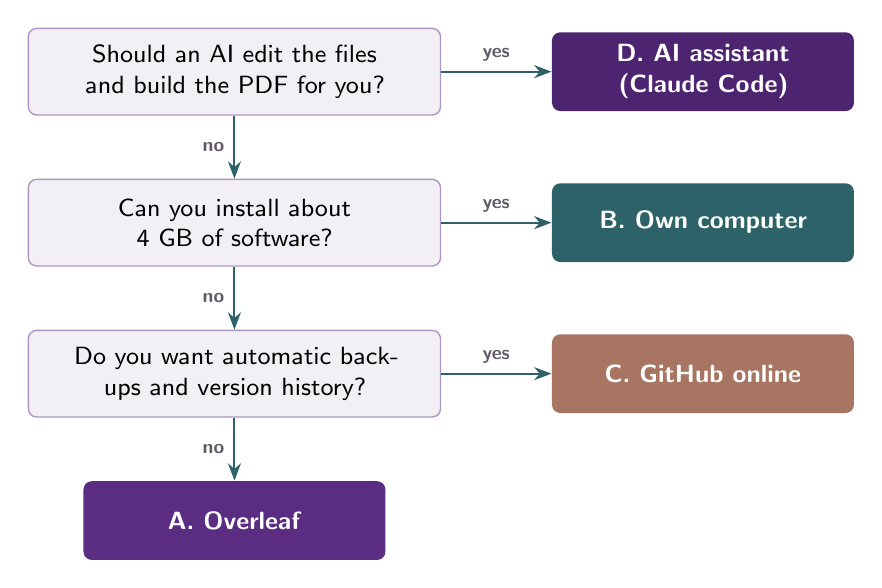
\begin{tikzpicture}[
  q/.style={rectangle,rounded corners=3pt,fill=iuclav,draw=iucpurple!50,line width=0.5pt,
    align=center,text width=50mm,minimum height=11mm,font=\sffamily\small},
  a/.style={rectangle,rounded corners=3pt,fill=#1,text=white,align=center,
    text width=36mm,minimum height=10mm,font=\sffamily\small\bfseries},
  lab/.style={font=\sffamily\scriptsize\bfseries,text=iucgrey},
  arr/.style={-{Stealth[length=2.2mm]},line width=0.7pt,draw=iucteal},
  node distance=8mm and 14mm]
  \node[q] (q1) {Should an AI edit the files and build the PDF for you?};
  \node[a=iucdeep,right=of q1] (d) {D.\ AI assistant (Claude Code)};
  \node[q,below=of q1] (q2) {Can you install about 4 GB of software?};
  \node[a=iucteal,right=of q2] (b) {B.\ Own computer};
  \node[q,below=of q2] (q3) {Do you want automatic backups and version history?};
  \node[a=iucrose!85!black,right=of q3] (c) {C.\ GitHub online};
  \node[a=iucpurple,below=of q3] (a) {A.\ Overleaf};
  \draw[arr] (q1) -- node[lab,above]{yes} (d);
  \draw[arr] (q1) -- node[lab,left]{no} (q2);
  \draw[arr] (q2) -- node[lab,above]{yes} (b);
  \draw[arr] (q2) -- node[lab,left]{no} (q3);
  \draw[arr] (q3) -- node[lab,above]{yes} (c);
  \draw[arr] (q3) -- node[lab,left]{no} (a);
\end{tikzpicture}
\caption{Choosing a workflow; read from top to bottom.}
\label{fig:choose}
\end{figure}

Whatever the workflow, any AI chat assistant can still help with individual
tasks such as converting tables or explaining errors (Section~\ref{sec:ai}).

% ===========================================================================
\section{Getting the template}\label{sec:get}
% ===========================================================================

The template is published at \repo. Never write your thesis in the original
repository; make your own copy first.

\subsection{Download a ZIP file}

Use this for Overleaf or your own computer.
\begin{enumerate}
  \item Open \repo{} in a web browser.
  \item Click the green \ui{Code} button, then \ui{Download ZIP}.
  \item Save the file. Keep it zipped if you will upload it to Overleaf;
        otherwise, extract it to a folder such as \file{Documents/thesis}.
\end{enumerate}

\subsection{Create your own GitHub repository}

Use this for GitHub online (Section~\ref{sec:github}) and Claude Code
(Section~\ref{sec:claudecode}). A free GitHub account is needed.
\begin{enumerate}
  \item Open \repo{} and sign in to GitHub.
  \item Click \ui{Use this template}\then\ui{Create a new repository}. If the
        button is not shown, click \ui{Fork} instead.
  \item Name the repository, for example \file{my-thesis}.
  \item Select \ui{Private} so that only you, and people you invite, can see it.
  \item Click \ui{Create repository}.
\end{enumerate}

\begin{warnbox}[Keep unpublished work private]
Use a private repository for your thesis. Do not store passwords, participant
data, or confidential documents in it.
\end{warnbox}

\subsection{What the repository contains}

\begin{table}[htbp]
\caption{Contents of the template repository.}
\label{tab:files}
\small
\begin{tabularx}{\textwidth}{@{}>{\ttfamily}p{46mm}X>{\centering\arraybackslash}p{15mm}@{}}
\toprule
\normalfont\thd{File or folder} & \thd{Contents} & \thd{You edit} \\
\midrule
metadata.tex          & Title, name, matric number, address, degree, dates     & Yes \\
main.tex              & Order of the parts; document type on line~1             & Rarely \\
frontmatter/          & Acknowledgement, Abstrak, Abstract, optional pages     & Yes \\
chapters/             & \texttt{chapter1.tex} to \texttt{chapter5.tex}          & Yes \\
appendices/           & \texttt{appendixA.tex} and further appendices           & Yes \\
references.bib        & Reference entries in BibTeX format                     & Yes \\
figures/              & Images used in figures                                 & Yes \\
spine.tex             & Spine strip for the binder                             & No \\
iucthesis.cls         & The formatting rules                                   & No \\
latexmkrc, .vscode/, .github/ & Build settings for latexmk, VS Code, and GitHub & No \\
README.md, STUDENT\_GUIDE.md, docs/ & Documentation, including this manual     & No \\
\bottomrule
\end{tabularx}
\end{table}

\begin{figure}[htbp]
\centering
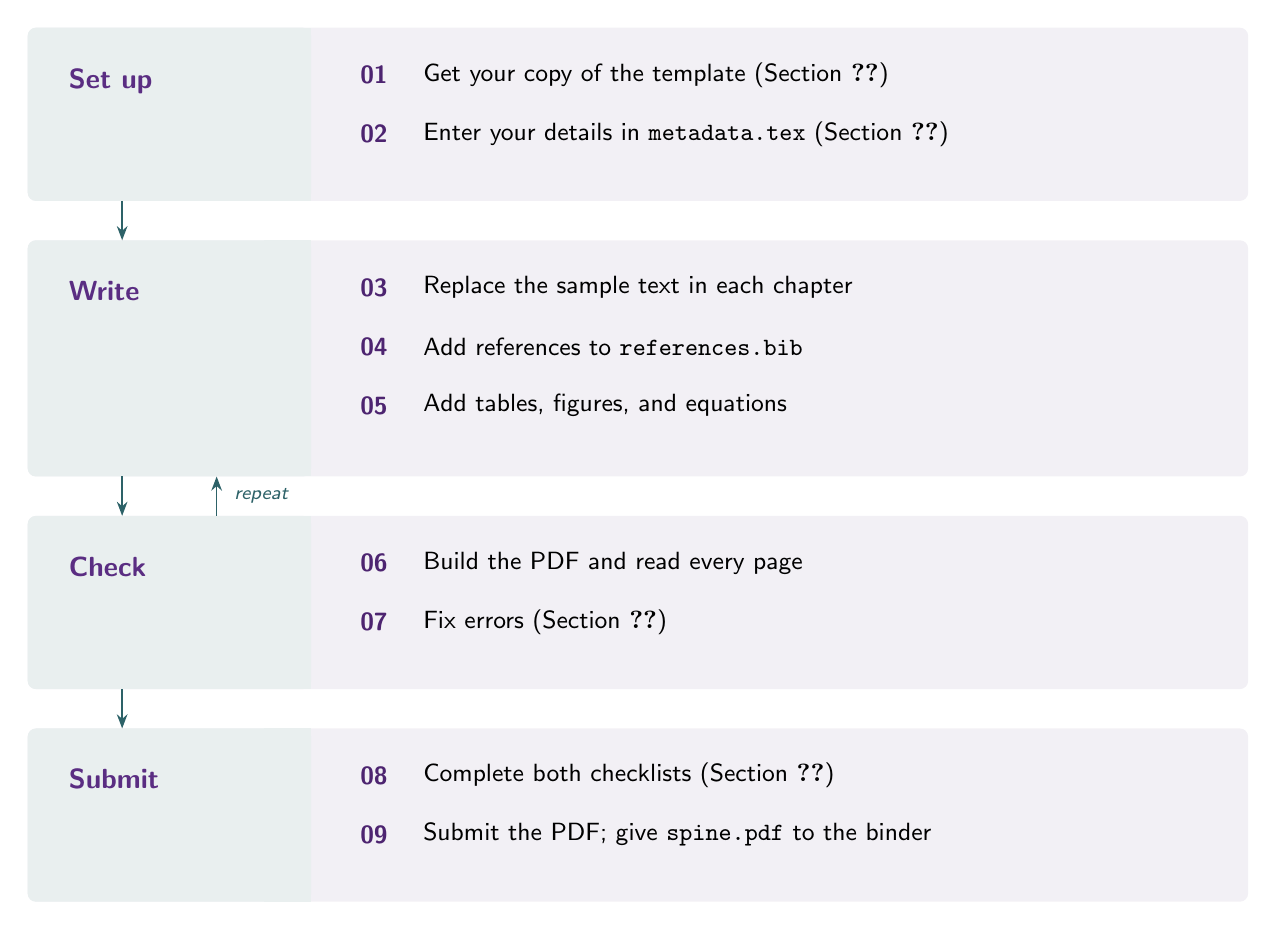
\begin{tikzpicture}[x=1mm,y=1mm,
  lab/.style={anchor=north west,font=\sffamily\bfseries\color{iucpurple},align=left},
  item/.style={anchor=west,font=\sffamily\small,align=left},
  num/.style={anchor=west,font=\sffamily\bfseries\small\color{iucdeep}},
  arr/.style={-{Stealth[length=1.8mm]},draw=iucteal,line width=0.6pt}]
  \foreach \y/\h/\name/\items in {
     0/22/Set up/{{01}/Get your copy of the template (Section~\ref{sec:get}),{02}/Enter your details in \texttt{metadata.tex} (Section~\ref{sec:details})},
    -27/30/Write/{{03}/Replace the sample text in each chapter,{04}/Add references to \texttt{references.bib},{05}/Add tables{,} figures{,} and equations},
    -62/22/Check/{{06}/Build the PDF and read every page,{07}/Fix errors (Section~\ref{sec:trouble})},
    -89/22/Submit/{{08}/Complete both checklists (Section~\ref{sec:checklist}),{09}/Submit the PDF; give \texttt{spine.pdf} to the binder}} {
    \fill[iuclav,rounded corners=3pt] (0,\y) rectangle (155,\y-\h);
    \fill[iuctealbg,rounded corners=3pt] (0,\y) rectangle (36,\y-\h);
    \fill[iuctealbg] (30,\y) rectangle (36,\y-\h);
    \node[lab] at (4,\y-4) {\name};
    \foreach \n/\t [count=\k] in \items {
      \node[num] at (41,\y-6-\k*7.5+7.5) {\n};
      \node[item] at (49,\y-6-\k*7.5+7.5) {\t};
    }
  }
  \draw[arr] (12,-22) -- (12,-27);
  \draw[arr] (12,-57) -- (12,-62);
  \draw[arr] (12,-84) -- (12,-89);
  \draw[arr,rounded corners=4pt] (24,-62) -- (24,-57);
  \node[font=\sffamily\scriptsize\itshape,text=iucteal,anchor=west] at (25,-59.5) {repeat};
\end{tikzpicture}
\caption{The writing cycle; read from top to bottom. Checking returns to writing
until the manuscript is complete.}
\label{fig:cycle}
\end{figure}

% ===========================================================================
\section{Working online with Overleaf}\label{sec:overleaf}
% ===========================================================================

Overleaf is a web-based LaTeX editor. Nothing is installed on your computer.

\begin{warnbox}[Check before writing]
The template maintainers have not yet tested the template on Overleaf. After
step~5, confirm that the sample thesis appears correctly before you add your
own content.
\end{warnbox}

\begin{enumerate}
  \item Download the template as a ZIP file (Section~\ref{sec:get}).
  \item Sign in to \href{https://www.overleaf.com}{\texttt{overleaf.com}}, or
        create a free account.
  \item Click \ui{New Project}\then\ui{Upload Project} and select the ZIP file.
  \item Open \ui{Menu} (top left). Under \textbf{Settings}, set \ui{Compiler}
        to \ui{XeLaTeX} and \ui{Main document} to \file{main.tex}.
  \item Click \ui{Recompile}. The sample thesis appears in the preview.
  \item Open files from the file list and replace the sample content
        (Sections~\ref{sec:details}--\ref{sec:appendices}).
  \item To submit, click the download icon above the preview to save the PDF.
\end{enumerate}

\textbf{Why XeLaTeX.} The template uses system fonts, which need the XeLaTeX
engine. With Overleaf's default pdfLaTeX setting, the build stops with the
message \emph{This class needs XeLaTeX or LuaLaTeX}.

\textbf{Build time.} Free Overleaf accounts limit how long one build may take.
A long thesis with many large images can exceed the limit. Compress images, or
change to Workflow~B or~C.

% ===========================================================================
\section{Working on your own computer}\label{sec:local}
% ===========================================================================

This workflow works offline and has no build limits. It needs a one-time
installation of a LaTeX system and an editor.

\subsection{Installing a LaTeX system}

\begin{table}[htbp]
\caption{Installing a LaTeX system.}
\label{tab:install}
\small
\begin{tabularx}{\textwidth}{@{}p{22mm}p{28mm}X@{}}
\toprule
\thd{System} & \thd{Distribution} & \thd{Notes} \\
\midrule
Windows & TeX Live & Run \texttt{install-tl-windows.exe} from \texttt{tug.org/texlive}; choose the full scheme. Allow 30--60 minutes. \\
macOS   & MacTeX   & Install \texttt{MacTeX.pkg} from \texttt{tug.org/mactex}. \\
Linux   & TeX Live & Use the installer from \texttt{tug.org/texlive}, or the distribution packages shown below. \\
\bottomrule
\end{tabularx}
\end{table}

On Debian or Ubuntu:
\begin{shell}
sudo apt install texlive-xetex texlive-latex-extra texlive-bibtex-extra \
  biber texlive-fonts-recommended fonts-texgyre latexmk
\end{shell}

\subsection{Visual Studio Code (recommended)}
\begin{enumerate}
  \item Install \href{https://code.visualstudio.com}{Visual Studio Code}.
  \item Open \ui{Extensions}, search for \textbf{LaTeX Workshop}, and click \ui{Install}.
  \item Choose \ui{File}\then\ui{Open Folder} and select the template folder.
  \item Open \file{main.tex} and click \ui{Build LaTeX project} (the green
        triangle, top right). Open the PDF with \ui{View LaTeX PDF}.
\end{enumerate}

The template includes \file{.vscode/settings.json}, which makes LaTeX Workshop
build with XeLaTeX and biber. Without it, the extension uses pdfLaTeX and the
build fails.

\subsection{TeXstudio}
TeXstudio is an all-in-one LaTeX editor. Set it up once:
\begin{enumerate}
  \item Choose \ui{Options}\then\ui{Configure TeXstudio}\then\ui{Build}.
  \item Set \ui{Default Compiler} to \ui{XeLaTeX} and
        \ui{Default Bibliography Tool} to \ui{Biber}, then click \ui{OK}.
  \item Open \file{main.tex} and press \ui{F5} to build and view.
\end{enumerate}

\subsection{Command line}
From the template folder:
\begin{shell}
latexmk main.tex        # build main.pdf
latexmk spine.tex       # build spine.pdf for the binder
latexmk -c              # remove temporary files
\end{shell}

\textbf{Fonts.} If Times New Roman and Arial Narrow are installed, as on most
Windows and macOS computers, the template uses them. Otherwise it uses the
metric-compatible free fonts TeX Gyre Termes and TeX Gyre Heros Condensed, and
notes the substitution in the log. Both give the same layout.

% ===========================================================================
\section{Working on GitHub}\label{sec:github}
% ===========================================================================

GitHub stores every version of your files. Each time you save a change, GitHub
builds the PDF automatically. No software is installed.

\begin{enumerate}
  \item Create your own private repository (Section~\ref{sec:get}).
  \item Open a file, such as \file{metadata.tex}, and click the pencil icon
        (\emph{Edit this file}).
  \item Make the change, click \ui{Commit changes\ldots}, add a short message
        such as ``Add my title'', and confirm with \ui{Commit changes}.
  \item Open the \ui{Actions} tab. Wait for the newest run to show a green tick;
        this takes about four minutes.
  \item Open the run and download \ui{iuc-thesis-pdf} under \textbf{Artifacts}.
        The ZIP file contains \file{main.pdf} and \file{spine.pdf}.
\end{enumerate}

\textbf{Images.} Open \file{figures/} and use \ui{Add file}\then\ui{Upload files}.

\textbf{Earlier versions.} Open a file and click \ui{History} to compare or
restore any earlier version.

\textbf{Failed builds.} A red cross means the build stopped. Open the run, then
the \ui{build} step, and look for lines starting with \texttt{!}.
Section~\ref{sec:trouble} lists common errors.

\textbf{Sharing with a supervisor.} In \ui{Settings}\then\ui{Collaborators},
invite your supervisor by GitHub username. They can read the files, see every
change, and comment, without email attachments.

\textbf{Build allowance.} Private repositories on free GitHub accounts include a
monthly allowance of build minutes. At about four minutes per build, it covers
several hundred builds a month.

% ===========================================================================
\section{Working with AI tools}\label{sec:ai}
% ===========================================================================

AI assistants can write and fix LaTeX, so that you can concentrate on content.
Table~\ref{tab:aitools} compares three ways to use them.

\begin{table}[htbp]
\caption{AI tools for the template.}
\label{tab:aitools}
\small
\begin{tabularx}{\textwidth}{@{}p{26mm}XXp{15mm}@{}}
\toprule
\thd{Tool} & \thd{What the AI does} & \thd{What you do} & \thd{Builds PDF} \\
\midrule
Claude Code     & Edits files, builds and checks the PDF, saves to GitHub & Describe changes in plain words & Yes \\
Claude Projects & Drafts LaTeX with your template and the Style Manual as context & Paste answers into your files & No \\
Any AI chat     & Answers one request at a time                           & Paste text in; copy LaTeX out     & No \\
\bottomrule
\end{tabularx}
\end{table}

\subsection{Claude Code}\label{sec:claudecode}

Claude Code works directly on your repository. It edits the files, builds the
PDF, checks the result, and saves the changes.

\begin{enumerate}
  \item Create your own GitHub repository (Section~\ref{sec:get}).
  \item Open \href{https://claude.ai/code}{\texttt{claude.ai/code}} and connect
        your GitHub account when asked.
  \item Start a session and select your thesis repository.
  \item Describe what you want, as in the examples below.
  \item Review the result, then ask Claude to commit and push the changes.
\end{enumerate}

\begin{promptbox}{Example requests for Claude Code}
Put my details in metadata.tex: title \ldots, name \ldots, matric number \ldots,
Master of Business Administration, submitted March 2027.\par
Replace section 1.1 with the text in the attached Word file.\par
Add the attached survey results to Chapter 4 as a table captioned
Respondent Demographics.\par
Build the PDF and show me the contents page and Chapter 4.
\end{promptbox}

Each new cloud session starts without LaTeX installed. Ask Claude once to
\emph{save a setup script that installs TeX Live for this environment}, so that
later sessions start ready.

\subsection{Claude Projects}

A Claude Project gives Claude permanent access to your template and the Style
Manual, so every answer follows them.

\begin{enumerate}
  \item On \texttt{claude.ai}, choose \ui{Projects}\then\ui{Create project}.
  \item In \textbf{Project knowledge}, choose \ui{+}\then\ui{GitHub} and select
        your repository. Include \file{README.md}, \file{iucthesis.cls},
        \file{main.tex}, \file{metadata.tex}, and your chapter files.
  \item Choose \ui{+}\then\ui{Upload} and add the Style Manual PDF.
  \item Paste the instructions below into \ui{Project instructions}.
  \item Work in chats inside the project; copy the LaTeX into your files.
\end{enumerate}

\textbf{Project instructions:}
\begin{prompttext}
I am writing an IUC thesis with the iucthesis LaTeX template in this project.
- Follow the IUC Style Manual and the template README.
- Use only \chapter, \section, and \subsection.
- Tables: \caption above the table; \tablenote{} for notes.
- Figures: \caption below the figure; \figuresource{} for the source.
- Every numbered equation needs \eqtitle{Short title}.
- Cite with \textcite{} or \parencite{} (APA 7); give BibTeX for new sources.
- Return LaTeX that I can paste straight into my chapter files.
\end{prompttext}

Project knowledge is a snapshot. After changing files on GitHub, click
\ui{Sync} on the GitHub item so that Claude sees the current version.

\subsection{Any AI chat assistant}

Claude, ChatGPT, Gemini, Copilot, and similar assistants can all help. Begin
each conversation by stating that you use the IUC \emph{iucthesis} LaTeX
template. Table~\ref{tab:prompts} gives requests that work well.

\begin{table}[htbp]
\caption{Prompt library for common tasks.}
\label{tab:prompts}
\small
\begin{tabularx}{\textwidth}{@{}p{30mm}X@{}}
\toprule
\thd{Task} & \thd{Request} \\
\midrule
Convert from Word   & \emph{Convert this text to LaTeX for the iucthesis template. Escape special characters and keep my citations as \textbackslash parencite\{key\}: [text]} \\
Build a table       & \emph{Turn this data into a LaTeX table for the iucthesis template, with booktabs rules, the caption [caption], and a \textbackslash tablenote: [data]} \\
Reference entries   & \emph{Create BibTeX entries for these references. Include DOIs, and protect acronyms and proper nouns in titles with braces: [references]} \\
Check citations     & \emph{List every \textbackslash parencite and \textbackslash textcite key in this chapter, and any key missing from this .bib file: [chapter] [bib]} \\
Explain an error    & \emph{My iucthesis LaTeX build stopped with this error. Explain it and show the fix: [error and nearby lines]} \\
Write an equation   & \emph{Write this formula as a numbered LaTeX equation with an \textbackslash eqtitle and a label: [formula]} \\
\bottomrule
\end{tabularx}
\end{table}

\subsection{Responsible use}

\begin{warnbox}[Candidates are responsible for their thesis]
\begin{itemize}[leftmargin=1.4em,itemsep=2pt,topsep=2pt]
  \item \textbf{Verify every reference.} AI tools can invent sources that do not
        exist. Confirm each one in the original publication or database.
  \item \textbf{Follow your programme's rules on AI use}, including any
        requirement to declare it. Ask your supervisor if unsure.
  \item \textbf{Protect confidential data.} Do not give participant data,
        unpublished results, or personal information to AI tools unless your
        ethics approval allows it.
  \item \textbf{Read everything the AI writes.} It can be wrong, and it does not
        know your research as you do.
\end{itemize}
\end{warnbox}

% ===========================================================================
\section{Entering your details}\label{sec:details}
% ===========================================================================

\subsection{The metadata file}

All personal details are entered once, in \file{metadata.tex}, and reused on
the cover, title page, declaration, PDF properties, and spine. Replace only the
text inside the braces \texttt{\{~\}}.

\begin{code}
\title{Strategic Leadership and Organisational\\ Performance in Higher Education}
\author{Nur Aina Binti Rahman}             % full registered name
\matricno{IUC/PhD/2026/001}
\address{Kuala Lumpur, Malaysia}
\degree{Doctor of Philosophy in Management} % full degree name
\degreeabbr{PhD}                            % abbreviation for the spine
\institution{Innovative University College}
\submissiondate{October 2026}              % month and year
\submissionyear{2026}                      % year on the spine
\declarationdate{23 October 2026}
\end{code}

Use \texttt{\textbackslash\textbackslash} inside \cmd{title} to choose where a
long title breaks, so that its lines are balanced (Style Manual~5.1).

\subsection{Thesis, dissertation, or research project}

Line~1 of \file{main.tex} sets the wording on the title page and in the
declaration. Use \texttt{thesis}, \texttt{dissertation}, or \texttt{project}:
\begin{code}
\documentclass[thesis]{iucthesis}
\end{code}

Figures~\ref{fig:title} and~\ref{fig:decl} show where each detail appears.

\begin{figure}[p]
\panelhead{Internal title page}{Source notes}
\centering
\begin{tikzpicture}[x=1mm,y=1mm]
  \samplepage{1}{20/30/92.5/128.5}
  \snote{1}{-6}{Title}{\cmd{title}\{\} in \texttt{metadata.tex}. 14~pt bold uppercase;
    \texttt{\textbackslash\textbackslash} balances the lines.}{87,-31.5}
  \snote{2}{-30}{Name}{\cmd{author}\{\}. Write it as registered, each word capitalised.}{67,-57}
  \snote{3}{-52}{Statement and degree}{Class option \texttt{thesis}, \texttt{dissertation},
    or \texttt{project}; \cmd{degree}\{\} in bold uppercase.}{80,-81.5}
  \snote{4}{-78}{Institution}{\cmd{institution}\{\}, preset to IUC.}{75,-105}
  \snote{5}{-100}{Submission date}{\cmd{submissiondate}\{\}: month and year.}{63,-127.5}
  \snote{6}{-122}{Pagination}{Automatic. Counted as Roman page~i; the number is
    hidden. Margins 60/40/40/25~mm.}{56,-140}
  \samplescale
\end{tikzpicture}
\caption{Title-page sample: \cmd{maketitlepage} in \file{main.tex}.}
\label{fig:title}
\end{figure}

\begin{figure}[p]
\panelhead{Author declaration}{Source notes}
\centering
\begin{tikzpicture}[x=1mm,y=1mm]
  \samplepage{2}{19/15/92.5/136}
  \snote{1}{-6}{Heading}{Created by \cmd{makedeclaration}. Centred, bold uppercase.}{69,-16.3}
  \snote{2}{-28}{Fixed wording}{Required by the Style Manual. The word \emph{thesis}
    follows the class option.}{62,-23.2}
  \snote{3}{-52}{Date}{\cmd{declarationdate}\{\} in \texttt{metadata.tex}.}{39,-38.6}
  \snote{4}{-76}{Candidate details}{\cmd{author}, \cmd{matricno}, and \cmd{address};
    sign above the line.}{87.5,-40}
  \snote{5}{-104}{Pagination}{Automatic. The declaration is Roman page~ii.}{57,-141}
  \samplescale
\end{tikzpicture}
\caption{Author-declaration sample.}
\label{fig:decl}
\end{figure}

\clearpage
% ===========================================================================
\section{Front matter and contents}\label{sec:front}
% ===========================================================================

Each front-matter page has its own file. Replace the sample text; the headings,
order, and page numbers are set by the template.

\begin{table}[htbp]
\caption{Front-matter files.}
\label{tab:front}
\small
\begin{tabularx}{\textwidth}{@{}>{\ttfamily}p{60mm}X@{}}
\toprule
\normalfont\thd{File} & \thd{Contents} \\
\midrule
frontmatter/acknowledgement.tex & Academic, financial, technical, and personal support \\
frontmatter/abstrak.tex         & Malay abstract, placed first; optional \cmd{keywords}\{\} \\
frontmatter/abstract.tex        & English abstract; optional \cmd{keywords}\{\} \\
frontmatter/dedication.tex      & Optional; enable it in \file{main.tex} \\
frontmatter/abbreviations.tex   & Optional list of abbreviations; enable it in \file{main.tex} \\
\bottomrule
\end{tabularx}
\end{table}

To enable an optional page, delete the \texttt{\%} at the start of its line in
\file{main.tex}:
\begin{code}
% \begin{dedication}
To my family.
\end{dedication}
     % delete the first % to include
\end{code}

The cover, title page, declaration, table of contents, and the lists of tables,
figures, equations, and appendices are generated. A list with no entries is
left out, together with its contents entry (Style Manual~4). Never edit the
contents page by hand: change the heading or caption in the source instead.

\begin{figure}[p]
\panelhead{Table of contents}{Source notes}
\centering
\begin{tikzpicture}[x=1mm,y=1mm]
  \samplepage{3}{19/15/92.5/136}
  \snote{1}{-6}{Generated}{\cmd{tableofcontents} in \texttt{main.tex}. Rebuilt on
    every build; never typed by hand.}{93,-23}
  \snote{2}{-30}{Front matter}{Each front-matter page with its Roman page number.
    Empty lists are left out.}{62,-36}
  \snote{3}{-54}{Chapter entries}{From \cmd{chapter}\{\}. Shown as
    CHAPTER~1:~TITLE, without a page number.}{47.5,-52.7}
  \snote{4}{-80}{Sections}{From \cmd{section}\{\}. Subsections are not listed
    (Style Manual~6.5).}{45,-93.4}
  \snote{5}{-106}{References and appendices}{From \cmd{printreferences} and the
    chapters after \cmd{appendix}.}{75,-108}
  \samplescale
\end{tikzpicture}
\caption{Table-of-contents sample.}
\label{fig:toc}
\end{figure}

\clearpage
% ===========================================================================
\section{Writing chapters}\label{sec:chapters}
% ===========================================================================

\subsection{Headings}

\begin{code}
\chapter{Literature Review}
\section{Leadership Theories}
\subsection{Transformational Leadership}
\end{code}

Write headings in title case; chapter titles are converted to uppercase. Only
these three levels are allowed (Style Manual~10.2): \cmd{subsubsection} stops
the build with an explanatory error. Do not end headings with a full stop.

\subsection{Paragraphs and special characters}

Type paragraphs normally. A blank line starts a new paragraph; a single line
break does not. Indentation, spacing, and justification are automatic, so do
not add blank lines or spaces to position text.

\begin{table}[htbp]
\caption{Characters that need a backslash, and other typing conventions.}
\label{tab:chars}
\small
\begin{tabularx}{\textwidth}{@{}p{34mm}>{\ttfamily}p{44mm}X@{}}
\toprule
\thd{To print} & \normalfont\thd{Type} & \thd{Why} \\
\midrule
\%  \quad \$ \quad \& \quad \# \quad \_ & \textbackslash\% \textbackslash\$ \textbackslash\& \textbackslash\# \textbackslash\_ & These characters are LaTeX commands \\
``quotation''            & `{}`quotation'{}'          & Two backticks open; two apostrophes close \\
45--60 (range)           & 45-{}-60                   & Two hyphens make an en dash \\
Table~4.1 (no break)     & Table\textasciitilde\textbackslash ref\{\ldots\} & The tilde keeps the words on one line \\
\emph{italic}, \textbf{bold} & \textbackslash emph\{\ldots\}, \textbackslash textbf\{\ldots\} & Use sparingly (Style Manual~10.1) \\
\bottomrule
\end{tabularx}
\end{table}

\subsection{Lists and block quotations}

\begin{code}
\begin{itemize}         % use enumerate for 1, 2, 3
  \item First point
  \item Second point
\end{itemize}

\begin{quote}           % quotations of 40 words or more
Quoted text ... \parencite[p.~18]{smith2023}
\end{quote}
\end{code}

Block quotations are indented 1.27~cm and double-spaced, without quotation marks
(Style Manual~15.1).

\subsection{Adding and removing chapters}

The five default chapters can be combined or split (Style Manual~7). Add or
delete the matching line in \file{main.tex}, and create or delete the file:
\begin{code}
\include{chapters/chapter6}
\end{code}

\begin{figure}[p]
\panelhead{Chapter opening}{Source notes}
\centering
\begin{tikzpicture}[x=1mm,y=1mm]
  \samplepage{4}{19/15/92.5/136}
  \snote{1}{-6}{Chapter heading}{\cmd{chapter}\{Introduction\}. Number and title
    are automatic; the 40~mm top margin is applied.}{62.5,-21.5}
  \snote{2}{-32}{Section}{\cmd{section}\{Purpose\}: numbered 1.1, bold, left
    aligned.}{33,-35}
  \snote{3}{-56}{Body text}{Your paragraphs in \texttt{chapters/chapter1.tex}.
    Double spacing, 2~em indent, and 6~pt after are automatic.}{92.5,-42}
  \snote{4}{-82}{Subsection}{\cmd{subsection}\{\}: numbered 1.3.1. The lowest
    permitted level.}{47.5,-78.4}
  \snote{5}{-108}{Pagination}{\cmd{mainmatter} in \texttt{main.tex} starts Arabic
    page~1 here.}{57,-141}
  \samplescale
\end{tikzpicture}
\caption{Chapter-opening sample.}
\label{fig:chapter}
\end{figure}

\clearpage
% ===========================================================================
\section{Tables, figures, and equations}\label{sec:floats}
% ===========================================================================

Tables, figures, and equations are numbered by chapter and listed automatically
(Style Manual~12--14). Give each a \cmd{label}, and refer to it with
\cmd{ref}, so that numbers update when material moves.

\subsection{Tables}
The caption goes \textbf{above} the table.
\begin{code}
\begin{table}[htbp]
  \caption{Respondent Demographics}
  \label{tab:demographics}
  \begin{tabular}{lcc}
    \toprule
    Group  & Number & Percentage \\
    \midrule
    Male   & 120    & 48\% \\
    Female & 130    & 52\% \\
    \bottomrule
  \end{tabular}
  \tablenote{Percentages are rounded.}
\end{table}
\end{code}

For a wide table, place the whole \texttt{table} environment between
\texttt{\textbackslash begin\{landscape\}} and
\texttt{\textbackslash end\{landscape\}}. For a table longer than a page, use
\texttt{longtable}, which repeats its heading row on each page.

\subsection{Figures}
Save the image in \file{figures/}. The caption goes \textbf{below} the figure.
\begin{code}
\begin{figure}[htbp]
  \includegraphics[width=0.8\textwidth]{figures/framework}
  \caption{Research Framework}
  \label{fig:framework}
  \figuresource{Adapted from Smith (2023).}
\end{figure}
\end{code}

\textbf{Image quality.} Use PDF or PNG for charts and diagrams, and JPG for
photographs. Export charts from Excel, SPSS, or R as PDF, or at 300~dpi, so that
they stay sharp in print (Style Manual~13.2).

\subsection{Equations}
\begin{code}
\begin{equation}
  y = \beta_0 + \beta_1 x + \varepsilon
  \eqtitle{Linear Regression Model}
  \label{eq:regression}
\end{equation}
\end{code}

\cmd{eqtitle} supplies the short title shown in the List of Equations
(Style Manual~14). Refer to the equation in the text as
\texttt{Equation\textasciitilde(\textbackslash ref\{eq:regression\})}.

\begin{figure}[p]
\panelhead{Tables and figures}{Source notes}
\centering
\begin{tikzpicture}[x=1mm,y=1mm]
  \samplepage{5}{19/15/92.5/136}
  \snote{1}{-6}{Cross-reference}{\texttt{Table\textasciitilde\textbackslash ref\{\ldots\}}:
    the number is filled in automatically.}{69.5,-41.2}
  \snote{2}{-26}{Table caption}{\cmd{caption}\{\} first, inside \texttt{table}:
    above the table, numbered 4.1.}{72.5,-46}
  \snote{3}{-46}{Rules}{\cmd{toprule}, \cmd{midrule}, \cmd{bottomrule}; no
    vertical lines.}{73.5,-53}
  \snote{4}{-66}{Table note}{\cmd{tablenote}\{\} after the table.}{69,-60}
  \snote{5}{-86}{Artwork}{\cmd{includegraphics} with an image from
    \texttt{figures/}.}{78,-95}
  \snote{6}{-110}{Caption and source}{\cmd{caption}\{\} after the image, then
    \cmd{figuresource}\{\}.}{77.5,-113}
  \samplescale
\end{tikzpicture}
\caption{Table and figure sample.}
\label{fig:floats}
\end{figure}

\clearpage
% ===========================================================================
\section{Citations and references}\label{sec:refs}
% ===========================================================================

Citations and the reference list follow APA 7th edition (Style Manual~15). You
type a command with the source's \emph{key}; the template prints the citation
and builds the list.

\subsection{Citing sources}

Table~\ref{tab:cite} shows the commands for common situations, with the output
produced by the template.

\begin{table}[htbp]
\caption{Citation commands and the output they produce.}
\label{tab:cite}
\small
\begin{tabularx}{\textwidth}{@{}>{\raggedright\arraybackslash}p{27mm}>{\ttfamily\raggedright\arraybackslash}p{66mm}>{\raggedright\arraybackslash}X@{}}
\toprule
\thd{Situation} & \normalfont\thd{Command} & \thd{Output} \\
\midrule
Narrative                    & \textbackslash textcite\{lamport1994\}            & Lamport (1994) \\
Parenthetical                & \textbackslash parencite\{lamport1994\}           & (Lamport, 1994) \\
Two authors                  & \textbackslash parencite\{creswell2018\}          & (Creswell \& Creswell, 2018) \\
Three or more authors        & \textbackslash textcite\{devlin2019\}             & Devlin et al.\ (2019) \\
Multiple sources             & \textbackslash parencite\{lamport1994,knuth1984\} & (Knuth, 1984; Lamport, 1994) \\
Page                         & \textbackslash parencite[p.\textasciitilde 18]\{lamport1994\} & (Lamport, 1994, p.~18) \\
Page range                   & \textbackslash parencite[pp.\textasciitilde 3-{}-5]\{creswell2018\} & (Creswell \& Creswell, 2018, pp.~3--5) \\
Same author, several years   & \textbackslash parencite\{smith2020,smith2023\}   & (Smith, 2020, 2023) \\
Same author and year         & \textbackslash parencite\{brown2022a,brown2022b\} & (Brown, 2022a, 2022b) \\
Group author, first use      & \textbackslash parencite\{apa2020\}               & (American Psychological Association [APA], 2020) \\
Group author, later use      & \textbackslash parencite\{apa2020\}               & (APA, 2020) \\
Secondary source             & \textbackslash parencite[Bandura, 1977, as cited in][]\{smith2023\} & (Bandura, 1977, as cited in Smith, 2023) \\
No author                    & \textbackslash parencite\{standards2024\}         & (``Template Standards,'' 2024) \\
No date                      & \textbackslash parencite\{iucguide\}              & (Innovative University College, n.d.) \\
\bottomrule
\end{tabularx}
\end{table}

\textit{Note.} The letters \emph{a} and \emph{b}, the abbreviation in square
brackets, and \emph{n.d.}\ are added automatically. A group abbreviation comes
from the \texttt{shortauthor} field of the entry. Personal communications are
cited in the text only, and typed directly, for example (A.~Rahman, personal
communication, March~5, 2026).

\subsection{Adding references}

Each source is an entry in \file{references.bib}. Google Scholar
(\ui{Cite}\then\ui{BibTeX}), Zotero, Mendeley, and EndNote export entries in
this format. The key on the first line, such as \texttt{smith2023}, is what you
cite. Common patterns:

\subsubsection*{Journal article}
\begin{bib}
@article{smith2023,
  author  = {Smith, Jane and Lee, Ahmad},
  title   = {Leadership in {Malaysian} higher education},
  journal = {Journal of Education},
  volume  = {12}, number = {3}, pages = {45--60},
  year    = {2023}, doi = {10.1234/abcd}
}
\end{bib}

\subsubsection*{Book and edited-book chapter}
\begin{bib}
@book{creswell2018,
  author = {Creswell, John W. and Creswell, J. David},
  title  = {Research design: {Qualitative}, quantitative, and mixed methods approaches},
  edition = {5}, publisher = {SAGE}, year = {2018}
}
@incollection{tan2021,
  author = {Tan, Mei Ling}, title = {Chapter title},
  editor = {Wong, Kevin}, booktitle = {Book title},
  pages = {10--25}, publisher = {Publisher}, year = {2021}
}
\end{bib}

\subsubsection*{Report, webpage, and thesis}
\begin{bib}
@report{moe2024,
  author = {{Ministry of Education Malaysia}}, title = {Report title},
  number = {5}, year = {2024}, url = {https://example.gov.my/report}
}
@online{iucguide,
  author = {{Innovative University College}}, title = {Page title},
  url = {https://example.edu.my/guide}       % no year gives n.d.
}
@phdthesis{ali2022,
  author = {Ali, Siti}, title = {Thesis title},
  school = {Innovative University College}, year = {2022}
}
\end{bib}

\subsection{Checking references}

\begin{itemize}
  \item \textbf{Protect capital letters.} The APA style sets titles in sentence
        case. Put proper nouns and acronyms in braces, for example
        \texttt{\{Malaysian\}} or \texttt{\{BERT\}}, or they will print in
        lowercase.
  \item \textbf{Group authors} take double braces, for example
        \texttt{\{\{Ministry of Education Malaysia\}\}}, so they are not read as
        a surname and given name.
  \item \textbf{Exported entries contain errors}, such as missing DOIs or
        ``et~al.''\ typed as an author. Check each entry against its source.
  \item \textbf{Only cited sources are listed.} An entry in
        \file{references.bib} that is never cited does not appear.
\end{itemize}

\begin{figure}[p]
\panelhead{References}{Source notes}
\centering
\begin{tikzpicture}[x=1mm,y=1mm]
  \samplepage{6}{19/15/92.5/136}
  \snote{1}{-6}{Heading}{\cmd{printreferences} in \texttt{main.tex}.
    Chapter-opening margins.}{63.5,-21.5}
  \snote{2}{-30}{Entries}{Generated from \texttt{references.bib}; only cited
    sources appear.}{92.5,-30}
  \snote{3}{-54}{Hanging indent}{1.27~cm hanging indent, double spacing, no
    extra space between entries.}{25.5,-34.3}
  \snote{4}{-80}{APA formatting}{Italics, sentence case, and punctuation are
    applied automatically.}{49,-38.4}
  \snote{5}{-106}{Order}{Sorted alphabetically by first author.}{19.3,-42.6}
  \samplescale
\end{tikzpicture}
\caption{References sample.}
\label{fig:refs}
\end{figure}

\clearpage
% ===========================================================================
\section{Appendices}\label{sec:appendices}
% ===========================================================================

Appendices follow the references (Style Manual~16). After \cmd{appendix} in
\file{main.tex}, each \cmd{chapter} becomes APPENDIX~A, APPENDIX~B, and so on,
with a 40~mm top margin, and is added to the contents page and the List of
Appendices.

\begin{code}
\appendix
\chapter{Additional Proofs or Materials}
\label{app:proofs}

Use appendices for supplementary derivations, implementation details, or
extended results.

\include{appendices/appendixB}   % add a line for each new appendix
\end{code}

To refer to an appendix from the text, give it a \cmd{label} and write, for
example, \texttt{Appendix\textasciitilde\textbackslash ref\{app:instrument\}}.

% ===========================================================================
\section{Building and checking}\label{sec:build}
% ===========================================================================

\subsection{Build again after large changes}

Page numbers, the contents page, lists, and cross-references are updated on the
following build. Overleaf, \texttt{latexmk}, VS Code, and GitHub repeat the
build automatically when needed. If \texttt{??} appears, or a list looks out of
date, build once more.

\subsection{Checking the margins}

Add \texttt{showframe} to line~1 of \file{main.tex} to draw the text area on
every page. All text, tables, figures, and captions must stay inside it
(Style Manual~8.1). Remove the option before submission.
\begin{code}
\documentclass[thesis,showframe]{iucthesis}
\end{code}

\subsection{The spine}

Building \file{spine.tex} produces \file{spine.pdf}: the hardbound spine in the
Style Manual format, with the name, degree abbreviation, and year in 16~pt
bold uppercase and 60~mm clear at each end (Figure~\ref{fig:spine}). The binder
confirms the spine width, applies the award colour, and stamps the lettering in
gold. To change the width, edit the \cmd{setlength}\cmd{spinewidth}\{16mm\}
line in \file{spine.tex}.

\begin{figure}[htbp]
\centering
\begin{tikzpicture}[x=1mm,y=1mm]
  \node[inner sep=0pt,draw=black,line width=0.3pt] (sp) at (0,0)
    {
\includegraphics[angle=90,width=148.5mm]{spine-sample}};
  \draw[{Stealth[length=1.5mm]}-{Stealth[length=1.5mm]},iucgold!70!black,line width=0.4pt]
    ($(sp.south west)+(0,-3)$) -- node[below,font=\sffamily\tiny,text=iucgrey]{60 mm clear}
    ($(sp.south west)+(30,-3)$);
  \draw[{Stealth[length=1.5mm]}-{Stealth[length=1.5mm]},iucgold!70!black,line width=0.4pt]
    ($(sp.south east)+(-30,-3)$) -- node[below,font=\sffamily\tiny,text=iucgrey]{60 mm clear}
    ($(sp.south east)+(0,-3)$);
\end{tikzpicture}
\caption{Spine strip from \file{spine.tex}, rotated to read from left to right,
at 50\% scale. The 16~mm width is an example; the binder sets the actual width.}
\label{fig:spine}
\end{figure}

\subsection{Final PDF}

Name the file clearly, for example \file{StudentID\_Surname\_Thesis.pdf}
(Style Manual~17). Fonts are embedded automatically. Read every page at full
size before submitting.

% ===========================================================================
\section{Troubleshooting}\label{sec:trouble}
% ===========================================================================

LaTeX stops at the first serious problem and prints a message beginning with
\texttt{!}, with the file and line number. Table~\ref{tab:trouble} lists the
usual causes.

\begin{table}[htbp]
\caption{Common error messages and their fixes.}
\label{tab:trouble}
\small
\begin{tabularx}{\textwidth}{@{}>{\raggedright\arraybackslash}p{46mm}>{\raggedright\arraybackslash}X>{\raggedright\arraybackslash}X@{}}
\toprule
\thd{Message or symptom} & \thd{Usual cause} & \thd{Fix} \\
\midrule
\texttt{This class needs XeLaTeX} & pdfLaTeX selected & Select XeLaTeX (Sections~\ref{sec:overleaf}, \ref{sec:local}) \\
\texttt{Missing \$ inserted} & \texttt{\_} or \texttt{\^{}} in normal text & Type \texttt{\textbackslash\_} or \texttt{\textbackslash\^{}\{\}} \\
Rest of a line missing & \texttt{\%} begins a comment & Type \texttt{\textbackslash\%} \\
\texttt{Missing \}} or \texttt{Runaway argument} & An unclosed \texttt{\{} & Close the brace \\
\texttt{Undefined control sequence} & Misspelt command & Check the spelling after \texttt{\textbackslash} \\
\texttt{Citation `\ldots' undefined} & Key not in \file{references.bib} & Check the key; build again \\
\texttt{??} instead of a number & References not yet updated & Build again \\
\texttt{\textbackslash subsubsection is not permitted} & A fourth heading level & Use \cmd{subsection} \\
\texttt{File `\ldots' not found} & Wrong image name or folder & Check the name and the \file{figures/} folder \\
Title printed in lowercase & Unprotected capitals in \file{.bib} & Put the word in braces \\
New entry missing from a list & Lists update on the next build & Build again \\
Font substitution warning & Times New Roman not installed & None; the free equivalent is used \\
\bottomrule
\end{tabularx}
\end{table}

\textbf{Isolating a problem.} Undo the most recent change and build again. If
the build succeeds, the problem is in that change. Otherwise, copy the error
and the lines around it into an AI assistant (Section~\ref{sec:ai}), or report
it on the template's GitHub page under \ui{Issues}.

\clearpage
% ===========================================================================
\section{Quick reference}\label{sec:quick}
% ===========================================================================

\begin{table}[htbp]
\caption{Command quick reference.}
\label{tab:quick}
\small
\begin{tabularx}{\textwidth}{@{}>{\ttfamily\raggedright\arraybackslash}p{76mm}>{\raggedright\arraybackslash}X@{}}
\toprule
\normalfont\thd{Command} & \thd{Result} \\
\midrule
\textbackslash chapter\{Title\}                  & New chapter on a new page \\
\textbackslash section\{Title\}                  & Section, e.g.\ 1.1 \\
\textbackslash subsection\{Title\}               & Subsection, e.g.\ 1.1.1 \\
\textbackslash textcite\{key\}                   & Lamport (1994) \\
\textbackslash parencite\{key\}                  & (Lamport, 1994) \\
\textbackslash parencite[p.\textasciitilde 5]\{key\} & (Lamport, 1994, p.~5) \\
\textbackslash label\{x\}\quad \textbackslash ref\{x\} & Name an item; print its number \\
\textbackslash tablenote\{\ldots\}               & \emph{Note.} line below a table \\
\textbackslash figuresource\{\ldots\}            & \emph{Source:} line below a figure \\
\textbackslash eqtitle\{\ldots\}                 & Title in the List of Equations \\
\textbackslash keywords\{\ldots\}                & Keywords below an abstract \\
\textbackslash begin\{quote\}\ldots              & Block quotation (40 or more words) \\
\textbackslash begin\{itemize\} \textbackslash item\ldots & Bullet list \\
\textbackslash begin\{landscape\}\ldots          & Landscape page \\
\textbackslash appendix                          & Following chapters become appendices \\
showframe (class option)                         & Draw the text area for checking \\
\bottomrule
\end{tabularx}
\end{table}

% ===========================================================================
% Checklist form (no header, no strip)
% ===========================================================================
\clearpage
\iucstripfalse
\thispagestyle{empty}
\refstepcounter{section}
\addcontentsline{toc}{section}{\protect\numberline{\thesection}Template setup and build checklist}
\label{sec:checklist}
\newgeometry{top=18mm,bottom=18mm,left=20mm,right=20mm}
\begin{center}
  {\sffamily\bfseries\large INNOVATIVE UNIVERSITY COLLEGE\par}\vspace{6pt}
  {\sffamily\bfseries\Large TEMPLATE SETUP AND BUILD CHECKLIST\par}\vspace{4pt}
  {\sffamily\small Candidate self-check before the formatting review\par}
\end{center}
\vspace{4pt}
\fcolorbox{iucpurple}{white}{\parbox{\dimexpr\textwidth-2\fboxsep-2\fboxrule}{\small
  \textbf{Template checks only.} This page supplements, and does not replace, the
  Final Manuscript Submission Checklist in the Style Manual (Section~18).}}

\vspace{10pt}
{\large\bfseries Candidate and manuscript\par}\vspace{6pt}
\renewcommand\arraystretch{1.9}
\begin{tabularx}{\textwidth}{@{}p{30mm}X p{22mm}p{32mm}@{}}
\textbf{Name:} & \hrulefill & \textbf{Matric no.:} & \hrulefill \\
\textbf{Programme:} & \hrulefill & \textbf{Degree:} & \hrulefill \\
\end{tabularx}
\begin{tabularx}{\textwidth}{@{}p{32mm}X@{}}
\textbf{Workflow:} & \cbox~Overleaf\quad \cbox~Own computer\quad \cbox~GitHub\quad \cbox~AI-assisted \\
\textbf{Document type:} & \cbox~Thesis\quad \cbox~Dissertation\quad \cbox~Research project \\
\end{tabularx}
\renewcommand\arraystretch{1.2}

\vspace{8pt}
{\large\bfseries Template checklist\par}\vspace{4pt}
{\small
\begin{tabularx}{\textwidth}{@{}X>{\centering\arraybackslash}p{14mm}@{}}
\toprule
\textbf{Item} & \textbf{Done} \\
\midrule
\texttt{metadata.tex} matches the registration records: title, name, matric number, degree. & \cbox \\
The document type on line 1 of \texttt{main.tex} is correct.                     & \cbox \\
No sample text from the template remains in any file.                            & \cbox \\
The Abstrak and Abstract report the same study, with matching terms and numbers. & \cbox \\
Headings use only \cmd{chapter}, \cmd{section}, and \cmd{subsection}.            & \cbox \\
Every table, figure, and appendix is referred to in the text with \cmd{ref}.     & \cbox \\
Every numbered equation has an \cmd{eqtitle}.                                    & \cbox \\
Every citation resolves; no \texttt{??} or undefined citations remain.           & \cbox \\
Every reference has been checked against its source, including any found with AI. & \cbox \\
Proper nouns and acronyms in reference titles print with correct capitals.       & \cbox \\
\texttt{showframe} has been removed, and nothing extends beyond the text area.   & \cbox \\
The final build completed without errors; every page has been read.              & \cbox \\
\texttt{spine.pdf} has been produced and checked against the title page.         & \cbox \\
\bottomrule
\end{tabularx}}

\vspace{14pt}
{\large\bfseries Candidate confirmation\par}\vspace{8pt}
\begin{tabularx}{\textwidth}{@{}p{44mm}X p{12mm}p{34mm}@{}}
\textbf{Candidate signature:} & \hrulefill & \textbf{Date:} & \hrulefill \\
\end{tabularx}
\restoregeometry
\clearpage

% ===========================================================================
% Back cover
% ===========================================================================
\thispagestyle{empty}
\begin{tikzpicture}[remember picture,overlay,x=1mm,y=1mm]
  \coordinate (NW) at (current page.north west);
  \coordinate (SW) at (current page.south west);
  \coordinate (SE) at (current page.south east);
  \fill[iucdeep] (SW) rectangle (current page.north east);
  \fill[iucpurple] (NW) rectangle ($(current page.north east)+(0,-76)$);
  \fill[iucteal] ($(SE)+(0,170)$) -- (SE) -- ($(SW)+(80,0)$) -- cycle;
  \draw[white!70!iucteal,line width=0.3pt] ($(SE)+(0,170)$) -- ($(SW)+(80,0)$);
  \fill[iucgold] ($(NW)+(18,-76)$) rectangle ($(NW)+(152,-77.4)$);
  \fill[iucteal!85!white] ($(NW)+(152,-76)$) rectangle ($(NW)+(178,-77.4)$);
  \fill[iucrose] ($(NW)+(178,-76)$) rectangle ($(NW)+(191,-77.4)$);
  \node[anchor=north west,inner sep=0pt] at ($(NW)+(18,-22)$)
    {
\includegraphics[width=105mm]{iuc-logo-white}};
  \node[anchor=north west,align=left,text=iuccream,
    font=\sffamily\bfseries\fontsize{22}{26}\selectfont]
    at ($(NW)+(17,-92)$) {\addfontfeatures{LetterSpace=3}THESIS TEMPLATE\\
      \addfontfeatures{LetterSpace=3}USER MANUAL};
  \node[anchor=north west,text=white,font=\sffamily\small]
    at ($(NW)+(18,-112)$) {Guide for Candidates, Supervisors, and Programme Staff};
  \node[anchor=north west,text=iucgold,font=\sffamily\scriptsize]
    at ($(NW)+(18,-120)$) {\addfontfeatures{LetterSpace=3}EDITION 1.0};
  \fill[iuccream,rounded corners=6pt] ($(SW)+(18,38)$) rectangle ($(SE)+(-14,76)$);
  \node[anchor=north west,text=iucdeep,font=\sffamily\bfseries\small]
    at ($(SW)+(27,69)$) {Template source and updates};
  \node[anchor=north west,text=iucdeep,font=\sffamily\small,text width=150mm]
    at ($(SW)+(27,62)$)
    {\texttt{github.com/fahimroslan/iucstyle\_latex}\\[3pt]
     The template class is distributed under the LaTeX Project Public License 1.3c.\\
     Formatting rules: IUC Thesis \& Dissertation Style Manual, Edition 3.0.};
  \node[anchor=south east,text=white,font=\sffamily\scriptsize]
    at ($(SE)+(-18,14)$) {INNOVATIVE UNIVERSITY COLLEGE};
  \fill[iucrose] (SW) rectangle ($(SE)+(0,3.5)$);
\end{tikzpicture}

\end{document}
